\chapter{Implementation and Experiment}
\label{chp:implexperiment}
Lorem ipsum dolor sit amet, consectetur adipiscing elit, sed do eiusmod tempor incididunt ut labore et dolore magna aliqua. Ut enim ad minim veniam, quis nostrud exercitation ullamco laboris nisi ut aliquip ex ea commodo consequat. Duis aute irure dolor in reprehenderit in voluptate velit esse cillum dolore eu fugiat nulla pariatur. Excepteur sint occaecat cupidatat non proident, sunt in culpa qui officia deserunt mollit anim id est laborum.

"Lorem ipsum dolor sit amet, consectetur adipiscing elit, sed do eiusmod tempor incididunt ut labore et dolore magna aliqua. Ut enim ad minim veniam, quis nostrud exercitation ullamco laboris nisi ut aliquip ex ea commodo consequat. Duis aute irure dolor in reprehenderit in voluptate velit esse cillum dolore eu fugiat nulla pariatur. Excepteur sint occaecat cupidatat non proident, sunt in culpa qui officia deserunt mollit anim id est laborum."


\section{Tribler integration}
As a proof of concept, credit mining system was implemented as a module in Tribler. Tribler was built using python, compatible with version 2.x and 3.x. At the time credit mining system implemented in Tribler, Tribler stil use WX as GUI (Graphical User Interface) framework. As for the future, Tribler will move its GUI to use Qt, starting version 7.0 onwards. All of those components made Tribler work cross platform (Linux, MacOS, and Windows).

In the prior work, some of the credit mining system code were implemented by \citeauthor{2015:creditmining:capota} and Egbert Bouman in his Tribler fork\footnote{\url{https://github.com/mihaic/tribler/tree/channel_boosting_new_exp}} instead of the main repository. This made the compatibility and stability between Tribler and credit mining system broke, thus make the system unusable. At this stage, the credit mining code was 1528 line long with 51 deletions.

% implemented in wx for GUI
\subsection{Contribution on software engineering}
As part of the software engineering process, the credit mining code need to be pass several steps before merged into main repository. First and foremost, is to open a Pull Request from forked repository to main. In Tribler, there are two main branch : \texttt{devel} for all new features and fixes, and \texttt{next} which contains bug fixes for the stable release. The pull request of first credit mining prototype was directed to \texttt{devel} branch as it is new feature at that point. Next phase is to work on the code itself by committing the work to the pull request. After that, other member of Tribler will review the implementation. One of the review material is the auto test report that executed by Jenkins\footnote{\url{http://jenkins.tribler.org/}}. The peer review process repeated until no other feedbacks. The lead developer will do a final review afterwards. After they gave OK sign, the commits need to be squashed and finally the pull request can be merged. Figure \ref{fig:cmpullrequest} shows the pull request that has been merged into Tribler main repository on \texttt{devel}.

\begin{figure}[h]
	\centering
	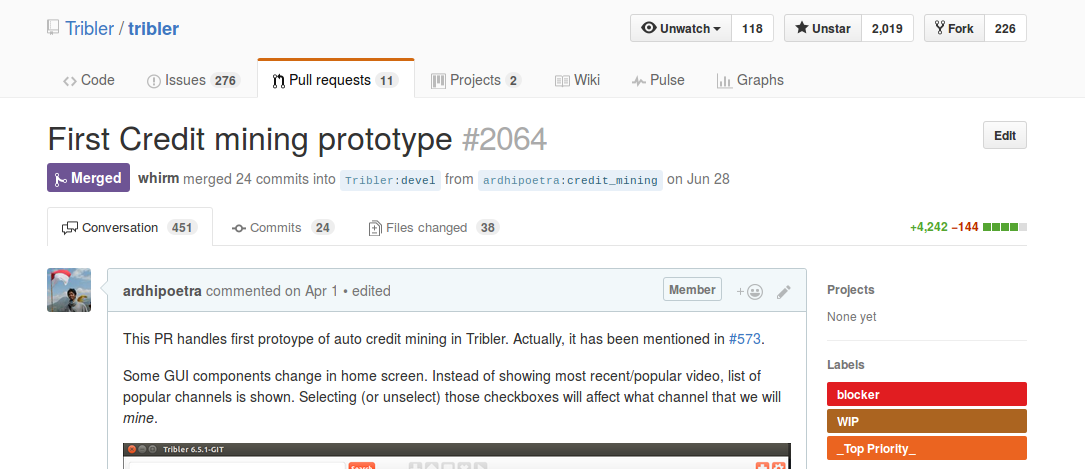
\includegraphics[width=\textwidth]{pics/cm_pr_crop.png}
	\caption[Merged pull request on credit mining prototype]{Merged pull request on credit mining prototype\footnotemark}.
	\label{fig:cmpullrequest}
\end{figure}

As shown in Figure \ref{fig:cmpullrequest}, the first credit mining prototype was heavily discussed by 6 other participants and more than 450 comments. It also takes almost 3 months to accommodate all the feedbacks and reviews. The coverage of this integration worth more than 4200 added lines and 140 deletions. The code portion is quite balanced with 1425 lines goes to GUI part of the code, 1290 lines to the credit mining system itself, 1160 lines to the tests, while the rest to other Tribler components to accommodate credit mining system. At the time of merging, credit mining system passed all the necessary test such and able to run in Linux, MacOS, and Windows (both 32 and 64 bit).

\footnotetext{Available in : \url{https://github.com/Tribler/tribler/pull/2064/}}
\subsection{Experience enhancement}
Credit mining system implementation is made publicly available for end user. It is important to encourage user to be as altruistic as possible. Therefore, in this system, we provide minimal interaction so non-altruistic user can be shown the effect of altruism and be convinced that this behavior is beneficial for both parties. In this part, we will elaborate the effort we have done on enhancing user experience of credit mining system on Tribler. As for comparison, Figure \ref{fig:oldcm} shows the only interface available from the previous work. In this version, it was not possible to add the mining sources except from the Tribler configuration file. 

\begin{figure}[h]
	\centering
	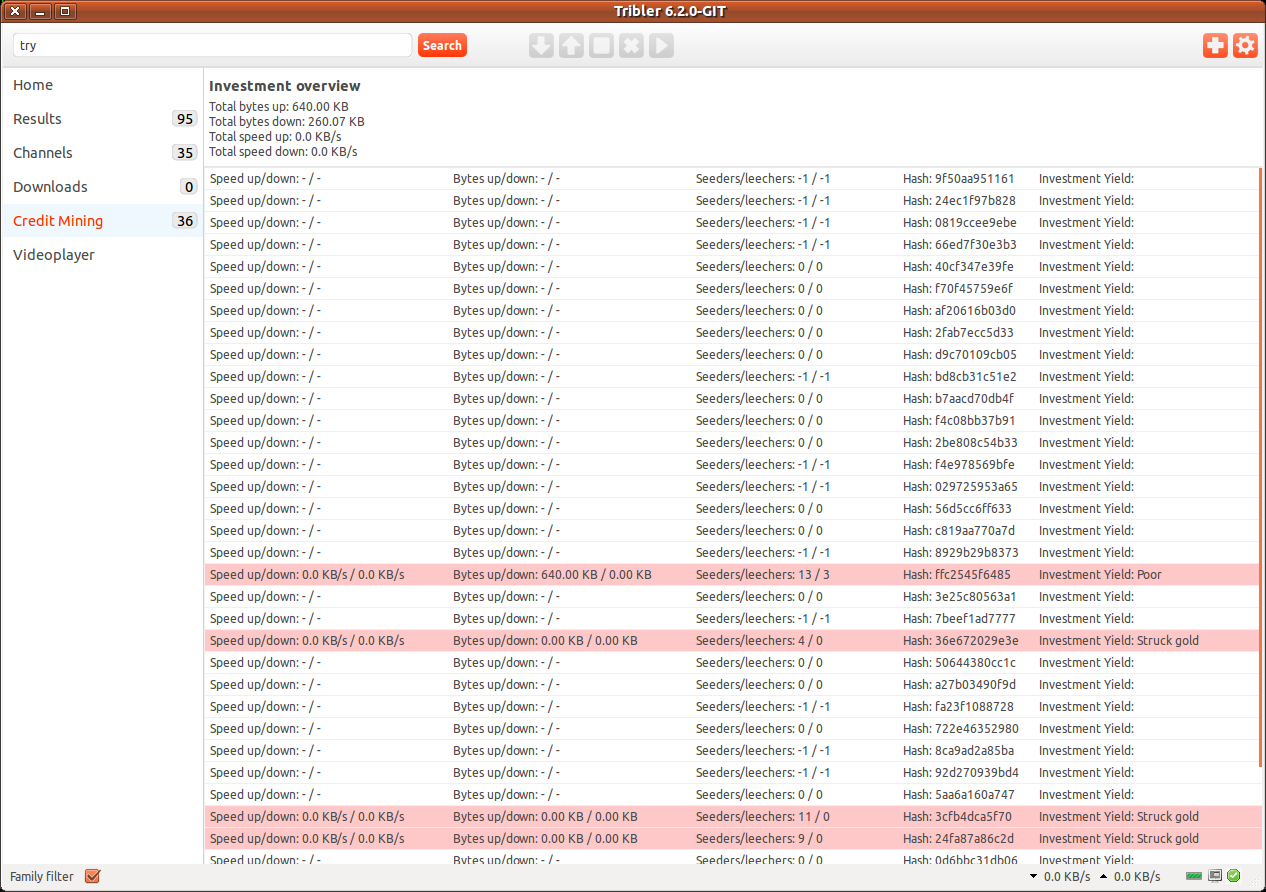
\includegraphics[width=0.8\textwidth]{pics/old_cm.png}
	\caption{The GUI for showing information from prior work \cite{2015:creditmining:capota}}.
	\label{fig:oldcm}
\end{figure}

\subsubsection{Graphical user interface revampment}

Start with the screen we called credit mining main window, it has similar interface compared with previous version. We improved the investment summary by adding more information of the mining source. The investment summary screen contains the swarms download/upload speed, amount of downloaded/uploaded, amount of seeder/leecher, and its identification. Figure \ref{fig:overview} shows this screen. In the same window, we also integrate an interface to easily add or remove mining sources. As mentioned in Section \ref{section:msource}, currently there are only 3 types of sources. Adding RSS and directory source can be done by clicking the upper left option. In the other hand, adding channel source can be done by put the mark in the check boxes in the source list. Figure \ref{fig:addsource} shows the example of adding directory source.

\begin{figure}[t!]
	\begin{adjustwidth}{-2.5cm}{}
		\begin{subfigure}[t]{0.6\textwidth}
			\centering
			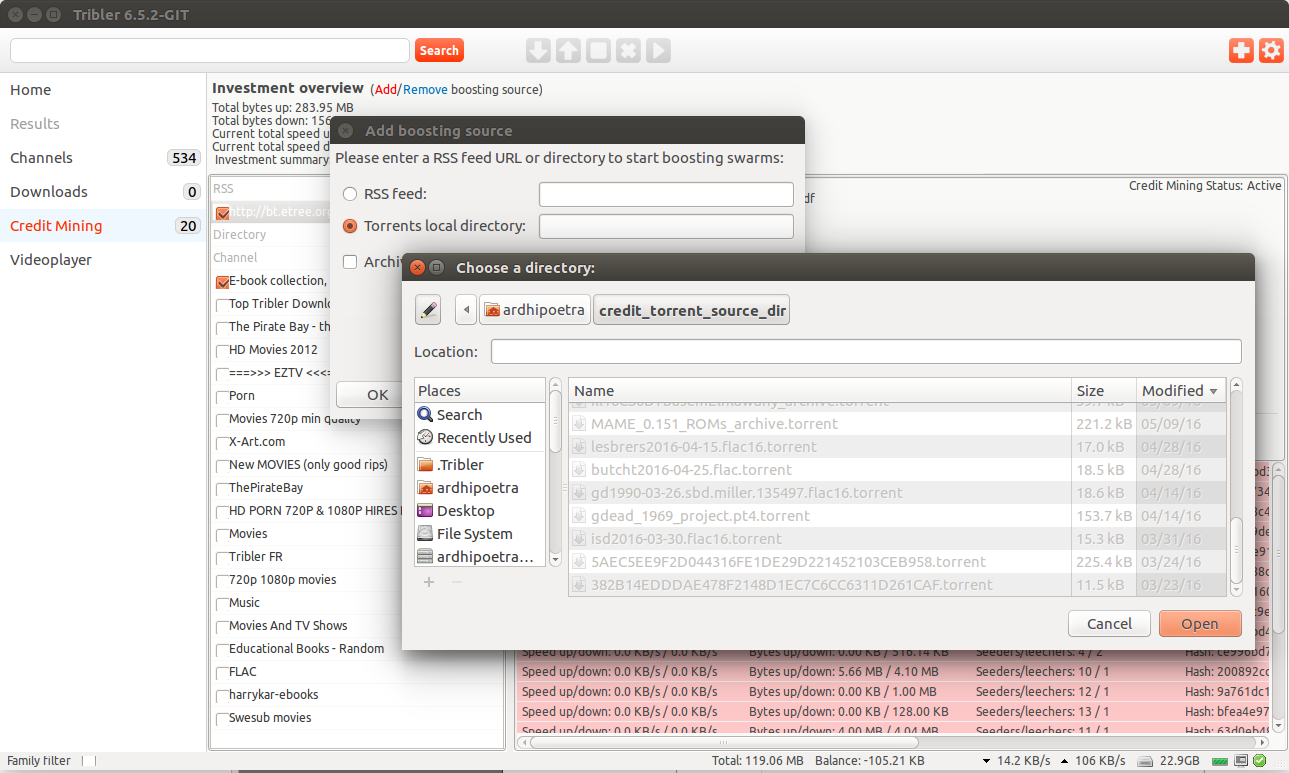
\includegraphics[width=\textwidth, height=6cm]{pics/add_source.png}
			\caption{The interface of adding mining source}.
			\label{fig:addsource}
		\end{subfigure}
		~
		\begin{subfigure}[t]{0.8\textwidth}
			\centering
			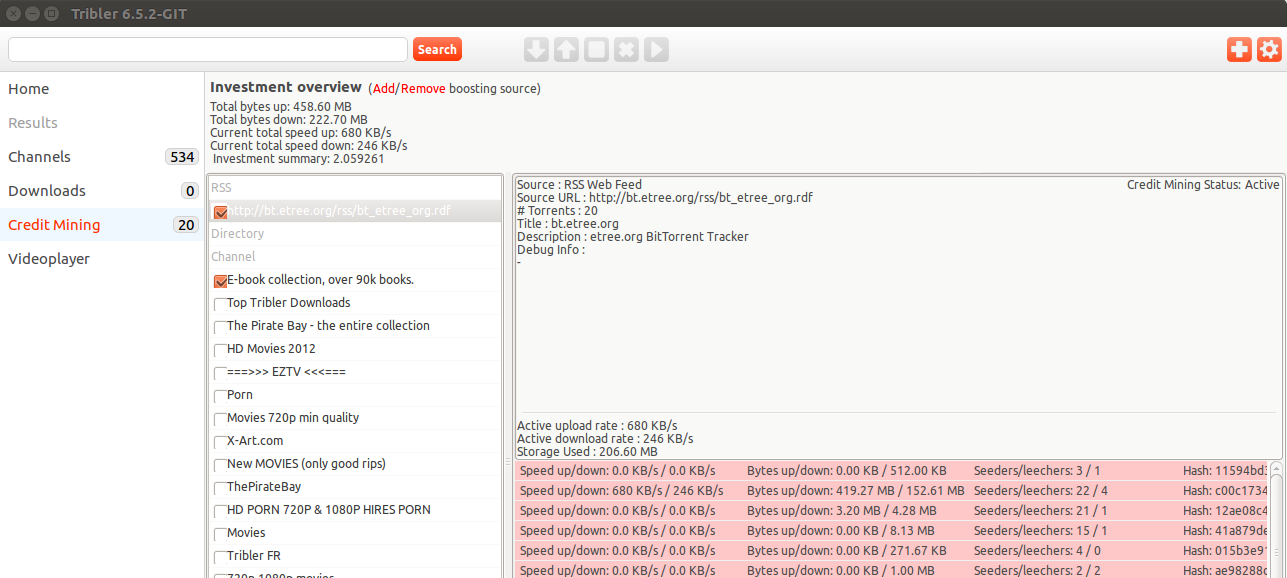
\includegraphics[width=\textwidth, height=6cm]{pics/overview_result.png}
			\caption{The investment overview}.
			\label{fig:overview}
		\end{subfigure}
		\caption{Credit mining main window.}
	\end{adjustwidth}
\end{figure}

Credit mining system is disabled by default in Tribler. Because it relates with automatically upload data, it might be concerned with privacy and security issue on end users. Therefore, a user must opt-in to enable credit mining. It can be done by flag the checkbox in Tribler settings window. After enabled, user need to restart Tribler to have the settings take effect. 

Activating credit mining module made the home screen of Tribler changed. We put several channels sorted by its popularity at the home screen as shown in Figure \ref{fig:homecm}. Channel is an integral part of Tribler which can be used to disseminate swarm information. This way, Tribler user do not need to leave the application to download new content. In home screen, user can simply click which channel he want to mine. This action will also be reflected in the credit mining main screen. To provide user with sufficient information, the popularity, shown by stars in the channel, and the random swarm that resides within that channel is showed. Moreover, user can also look for channel information if necessary. In this way, Tribler user have an easy access to mine a channel, which we strongly recommend.

\begin{figure}
	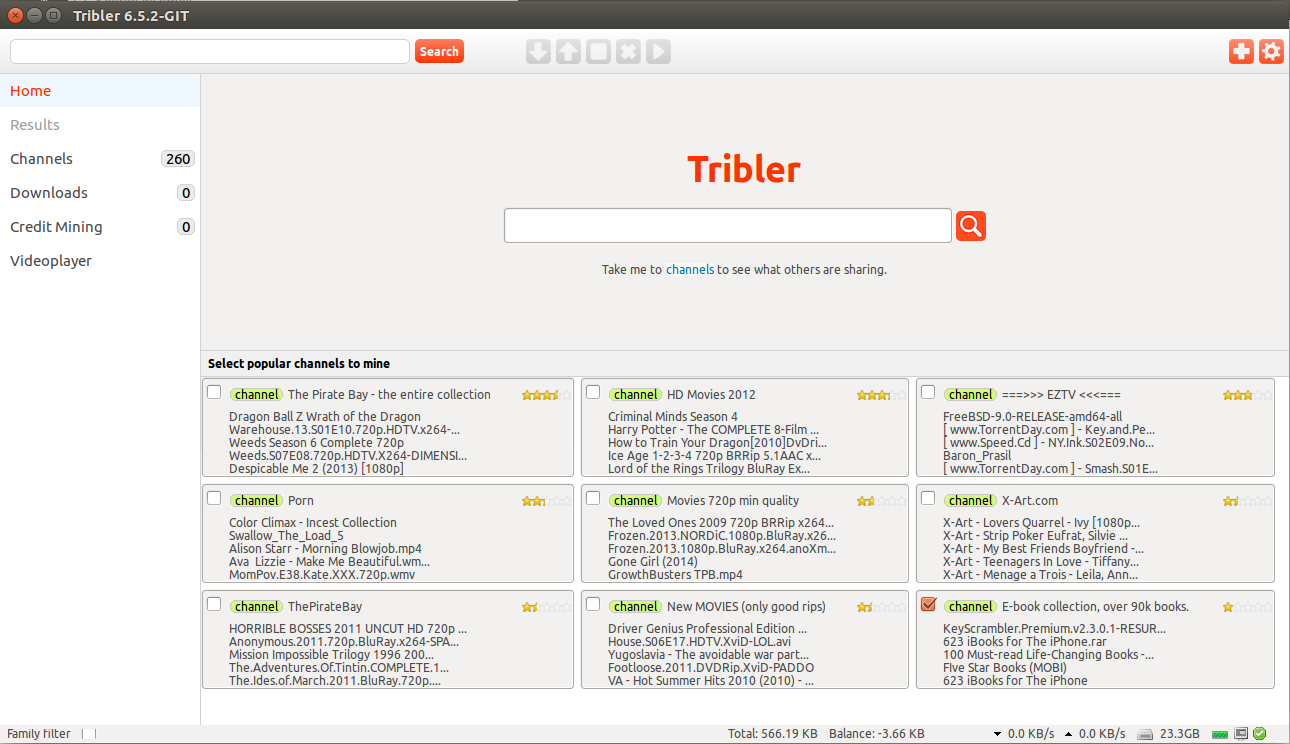
\includegraphics[width=\textwidth]{pics/home_channel.png}
	\caption{The home interface of Tribler with credit mining active}.
	\label{fig:homecm}
\end{figure}

In integrating with Tribler, we emphasize the simplicity to both interact with credit mining system and monitor gained credit. Especially to mine channel, two methods are introduced, both are by single-clicking the checkboxes in home screen (Figure \ref{fig:homecm}) or in credit mining main page (Figure \ref{fig:overview}). Although in the home screen only limited popular channel are shown, in credit mining main page this is not the case. After scrolled some content, if Tribler find another channel that has not been shown, it will append the list with that channel. Basically, it is an infinite list of channel with the upper bound the total number of channel available in Tribler environment. After the channel has been added to credit mining system, user can enable or disable it by another single click.

\subsubsection{User activity awareness}


\subsubsection{Libtorrent tuning}
settings in libtorrent to accommodate credit mining
\subsection{Anonymous and secure mining}
Tribler is well known for its anonymity and secure interface on top of \bt~ network. In 2014, Tribler published a specification on its anonymity feature\footnote{\url{https://github.com/Tribler/tribler/wiki/Anonymous-Downloading-and-Streaming-specifications}}. It uses Tor-like onion routing with purely distributed mechanism. A year later, \citeauthor{2015:tunnel:ruigrok} on his work completed the \textit{tunnel community} which emphasize end-to-end encryption in Tribler. This comes with several drawbacks. The most important one is performance degradation. Adding layers of privacy comes with increasing the amount of cryptography operation which slows down end-to-end downloading activity \cite{2015:tunnel:ruigrok}.


\begin{itemize}
	\item  usage of tunnel community
	\item  
\end{itemize}

\section{Gumby}
\subsection{Scenario and Configuration}

\section{Credit mining experiment}
\subsection{Comparing performance with prior work}
\subsubsection{New policy}
\subsection{Predownload hit capabilities}
\subsubsection{Torrent crawler}
\subsection{Experiment on user activity}

\section{Finding best parameters}
\subsection{Multiplier in scoring policy}
\subsection{Number of piece download}
\subsection{Peer translation accuracy}


